\documentclass{beamer}
\usepackage{../BigDataHeader}
\begin{document}
    \section{Statistics with Python}
    \subsection{Big Data at a Glance}
    \begin{frame}
        \frametitle{Big Data at a Glance}
        \begin{center}
            \Huge How to "describe" Big Data?
        \end{center}
    \end{frame}
    \begin{frame}
        \frametitle{Traditional View}
        \begin{itemize}
            \item Volume: The amount of data generated and stored
            \item Variety: The different types of data (structured, unstructured, semi-structured)
            \item Velocity: The speed at which data is generated and processed
            \item Veracity: The quality and accuracy of the data
            \item Value: The potential insights and benefits derived from the data
        \end{itemize}
    \end{frame}
    \begin{frame}
        \frametitle{Scientists' View}
        \begin{itemize}
            \item Data Science: The field of study that uses scientific methods, processes, algorithms, and systems to extract knowledge and insights from structured and unstructured data
            \begin{itemize}
                \item Data Statistics
                \item Data Modeling
            \end{itemize}
        \end{itemize}
    \end{frame}
    \subsection{Simple Statistics with Python}
    \subsubsection{Descriptive statistics}
    \begin{frame}
    \frametitle{Descriptive statistics with Pandas}
    \begin{itemize}
        \item \textbf{Descriptive Statistics} are informational statistical coefficients that describe, show, and summarize the collected data
        \item \textbf{Descriptive Statistics} usually answer three questions:
        \begin{itemize}
            \item Where is central?
            \item How broad is the base?
            \item How distributed is the data?
        \end{itemize}
    \end{itemize}
    \end{frame}

    \begin{frame}
        \frametitle{Where is the centre of the distribution?}
        \begin{itemize}
            \item \textbf{Mean}
            \begin{align*}
                x_{mean} = \frac{1}{n}\bigg(\sum_{i=1}^{n}x_{i}\bigg)
            \end{align*}
            \item \textbf{Median}
            \begin{align*}
                x_{median} = 
                \begin{cases}
                    x_{p}; p = \frac{n+1}{2} & \text{if $n$ is odd}\\
                    \frac{x_{p} + x_{p+1}}{2}; p = \frac{n}{2} & \text{if $n$ is even}
                \end{cases}
            \end{align*}
            \item \textbf{Mode}
            \begin{align*}
                x_{mode} = \text{most frequent data points}
            \end{align*}
        \end{itemize}
    \end{frame}
    \begin{frame}
        \frametitle{Where is the centre of the distribution?}
        \begin{center}
            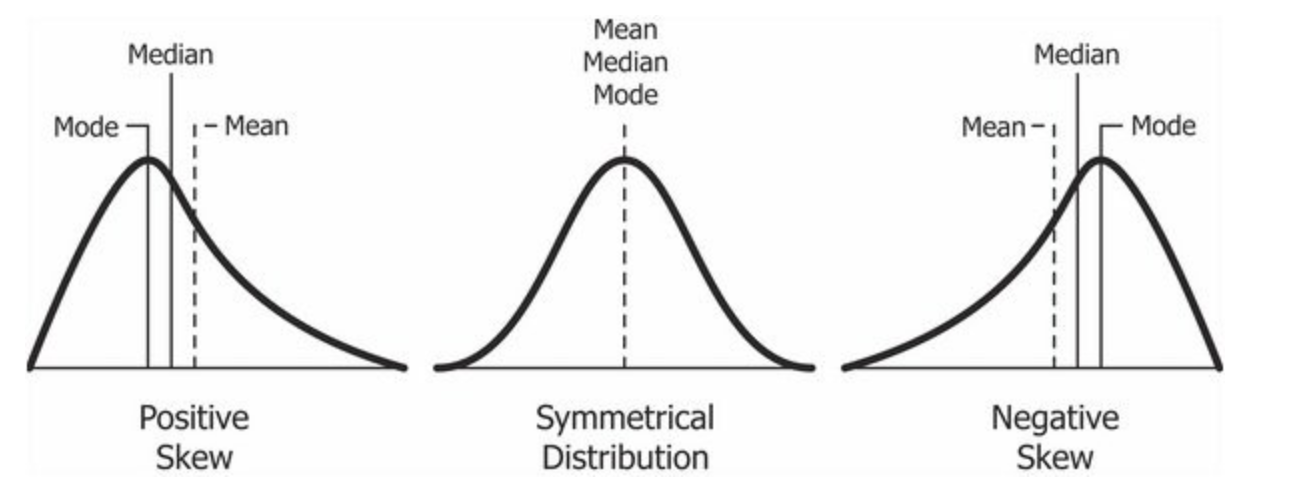
\includegraphics[width=0.8\textwidth]{figures/mmm.png}
        \end{center}
    \end{frame}

    \begin{frame}{How broad is the base?}
        \begin{itemize}
            \item \textbf{Variance}
            \begin{align*}
                Var(x) = \frac{1}{n}\sum_{i=1}^{n}(x_{i}-x_{mean})^{2}
            \end{align*}
            \item \textbf{Standard Deviation}
            \begin{align*}
                SD(x) = \sqrt{\frac{1}{n}\sum_{i=1}^{n}(x_{i}-x_{mean})^{2}}
            \end{align*}
        \end{itemize}
    \end{frame}
    \begin{frame}
        \frametitle{How broad is the base?}
        \begin{center}
            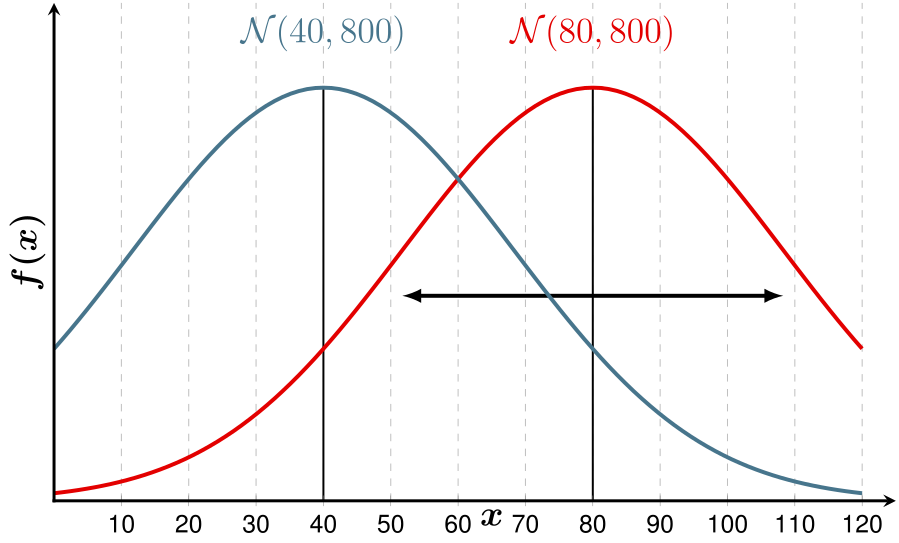
\includegraphics[width=0.8\textwidth]{figures/Variance.png}
        \end{center}
    \end{frame}

    \begin{frame}{How distributed is the data?}
        \begin{itemize}
            \item \textbf{Skewness}
            \begin{align*}
                Skew(x) = \frac{1}{n}\sum_{i=1}^{n}\frac{(x_{i}-x_{mean})^{3}}{SD(x)^{3}}
            \end{align*}
            \item \textbf{Kurtosis}
            \begin{align*}
                Kurt(x) = \frac{1}{n}\sum_{i=1}^{n}\frac{(x_{i}-x_{mean})^{4}}{SD(x)^{4}} - 3
            \end{align*}
        \end{itemize}
    \end{frame}

    \begin{frame}
        \frametitle{How distributed is the data?}
        \begin{center}
            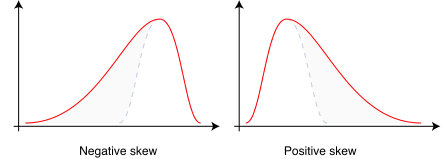
\includegraphics[width=0.7\textwidth]{figures/Skew.png}
            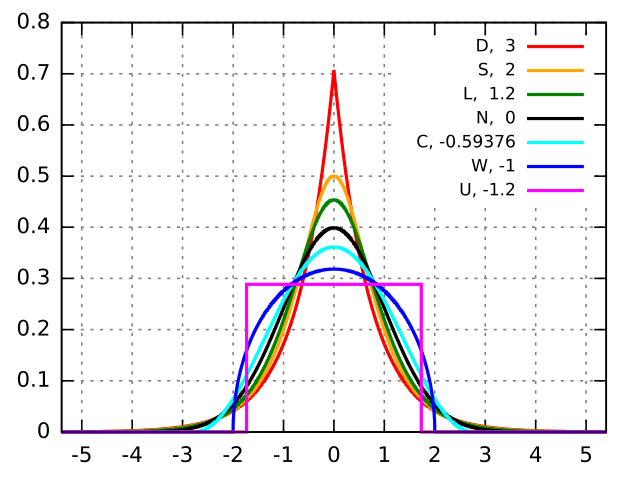
\includegraphics[width=0.5\textwidth]{figures/Kurtosis.png}
        \end{center}
    \end{frame}

    \begin{frame}{Example: Titanic}
        \begin{center}
            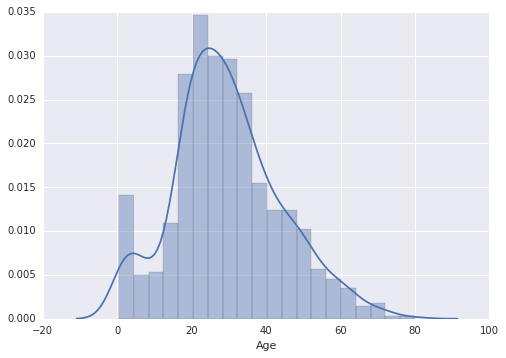
\includegraphics[width=0.8\textwidth]{figures/Titanic.png}
        \end{center}
    \end{frame}

    \begin{frame}{Example: Metro Health and Income}
        \begin{center}
            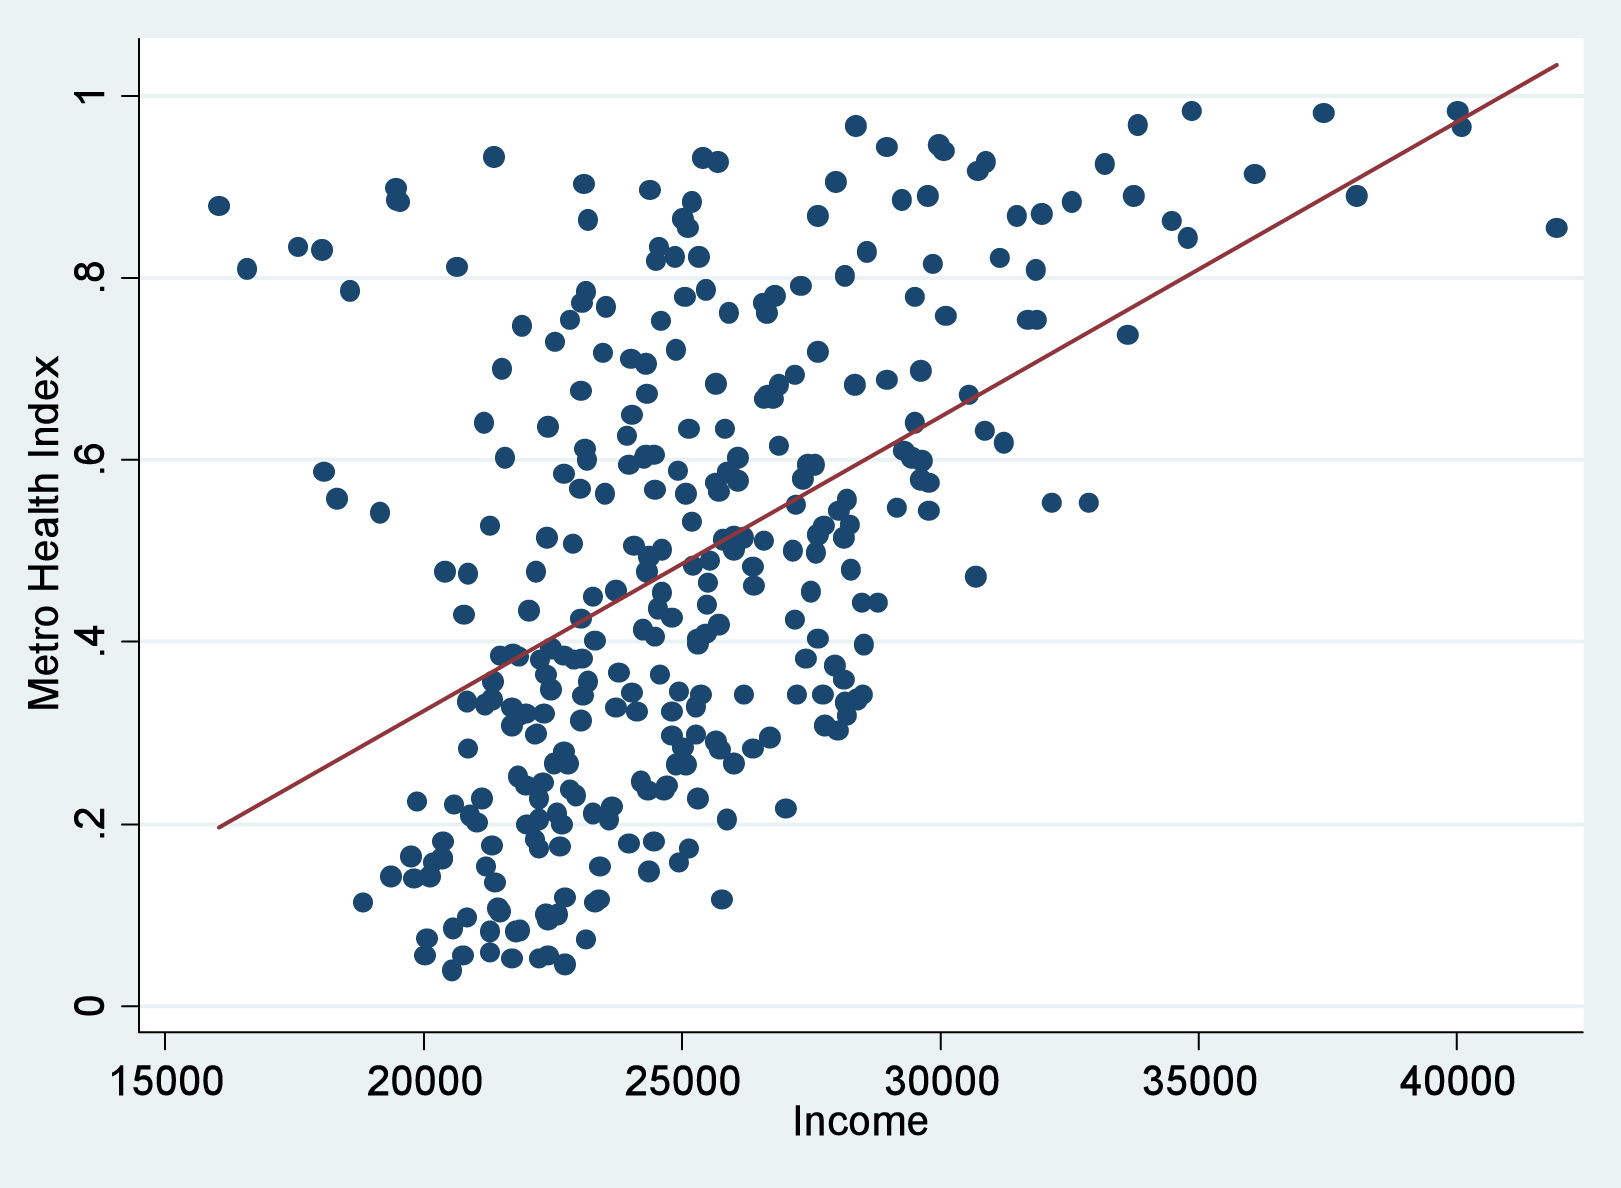
\includegraphics[width=0.8\textwidth]{figures/scatter_ex_atlanticcities.jpg}
        \end{center}
    \end{frame}
    \subsubsection{Calculating the Sum Using a For Loop}
    \begin{frame}[fragile]
        \frametitle{Calculating the Sum Using a For Loop}
        \begin{equation*}
            \sum_{i=0}^{n} x_{i}; x \in \mathbb{R}
        \end{equation*}
        \begin{itemize}
            \item Create a list with numerical values: \texttt{numbers = [1, 2, 3, 4, 5]}
            \item Initialize a variable to store the sum: \texttt{total = 0}
            \item Use a for loop to iterate over the list and add each element to the total:
        \end{itemize}
        \begin{lstlisting}[language=Python]
total = 0
for num in numbers:
    total += num
print("The sum is:", total)
        \end{lstlisting}
    \end{frame}

    \subsubsection{Calculating the Average of a Numerical List}
    \begin{frame}[fragile]
        \frametitle{Calculating the Average of a Numerical List}
        \begin{equation*}
            x_{mean}= \frac{\sum_{i=0}^{n} x_{i}; x \in \mathbb{R}}{n}
        \end{equation*}
        \begin{itemize}
            \item Use the previously calculated sum and divide it by the length of the list to get the average.
            \item The length of the list can be obtained using the \texttt{len()} function.
        \end{itemize}
        \begin{lstlisting}[language=Python]
average = total / len(numbers)
print("The average is:", average)
        \end{lstlisting}
    \end{frame}

    \subsubsection{Calculating the Biased Variance of a Numerical List}
    \begin{frame}[fragile]
        \frametitle{Calculating the Biased Variance of a Numerical List}
        \begin{equation*}
            Var(x) = \frac{1}{n}\sum_{i=1}^{n}(x_{i}-x_{mean})^{2}
        \end{equation*}
        \begin{itemize}
            \item Using the previously calculated average, the biased variance can be calculated.
            \item The \lstinline|x ** y| signifies the exponentiation of \lstinline|x| to the power of \lstinline|y|.
        \end{itemize}
        \begin{lstlisting}[language=Python]
total = 0
for num in numbers:
    total += (num - average) ** 2
variance = total / len(numbers)
print("The variance is:", variance)
        \end{lstlisting}
    \end{frame}
    \begin{frame}[fragile]
        \frametitle{About the Biased}
        \begin{itemize}
            \item The biased variance is the average of the squared differences from the mean.
            \item It is called "biased" because it divides by \lstinline|n|, which can underestimate the true variance in a sample.
            \item In practice, the unbiased variance is often used, which divides by \lstinline|n-1| instead of \lstinline|n|.
            \item The unbiased variance is a better estimate of the population variance when working with a sample.
        \end{itemize}
        \begin{equation*}
            Var(x) = \frac{1}{n-1}\sum_{i=1}^{n}(x_{i}-x_{mean})^{2}
        \end{equation*}
    \end{frame}

    \subsubsection{Inferential statistics}
    \begin{frame}{Inferential statistics}
        \begin{itemize}
            \item \textbf{Inferential Statistics} are statistical coefficients that allow us to make inferences about the population from the sample
            \item \textbf{Inferential Statistics} usually answer two questions:
            \begin{itemize}
                \item How likely is it that the sample is representative of the population?
                \item How likely is it that the sample is not representative of the population?
            \end{itemize}
        \end{itemize}
    \end{frame}
    \begin{frame}{How likely is it that the sample is representative of the population?}
        \begin{itemize}
            \item \textbf{Confidence Interval}
            \begin{align*}
                CI = x_{mean} \pm z_{\alpha/2}\frac{SD(x)}{\sqrt{n}}
            \end{align*}
            \item \textbf{Hypothesis Testing}
            \begin{align*}
                H_{0}: x_{mean} = x_{mean}^{\prime}\\
                H_{1}: x_{mean} \neq x_{mean}^{\prime}
            \end{align*}
        \end{itemize}
        \begin{center}
            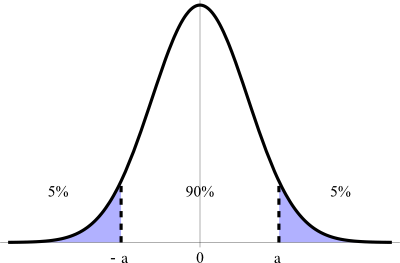
\includegraphics[width=0.4\textwidth]{figures/CI.png}
        \end{center}
    \end{frame}
    \begin{frame}{How likely is it that the sample is not representative of the population?}
        \begin{itemize}
            \item \textbf{P-value}
            \begin{align*}
                p = P(H_{0}|H_{1})
            \end{align*}
            \item \textbf{Type I Error}
            \begin{align*}
                \alpha = P(H_{0}|H_{1})
            \end{align*}
            \item \textbf{Type II Error}
            \begin{align*}
                \beta = P(H_{1}|H_{0})
            \end{align*}
        \end{itemize}
        \begin{center}
            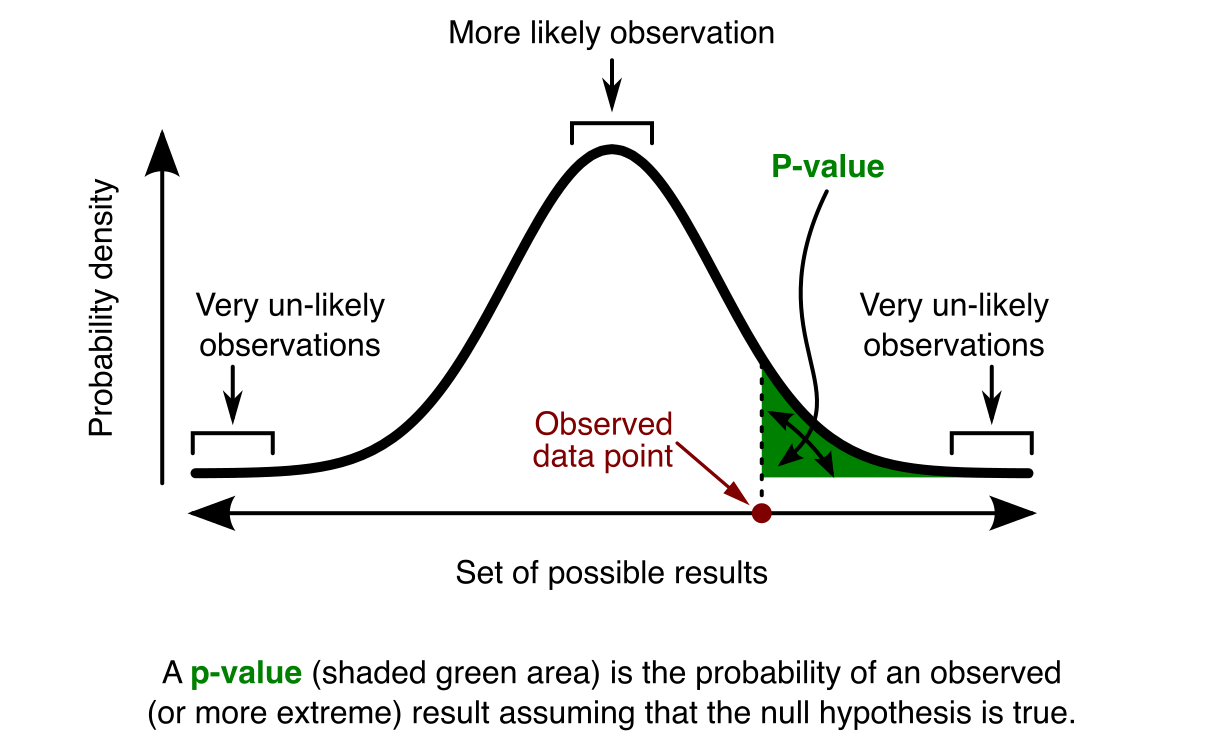
\includegraphics[width=0.4\textwidth]{figures/P-value.png}
        \end{center}
    \end{frame}

    \subsection{Advance Statistics with Python Frameworks}
    \begin{frame}[fragile]{Frameworks and Libraries}
        \begin{block}{What are Frameworks/Libraries?}
            Frameworks and libraries are a collection of software that automates functionalities for software developers. The difference between frameworks and libraries is that libraries are collections of packages that allow developers to control the application flow. In contrast, frameworks are packages of software designed with a singular purpose and with built-in basic application flow.
        \end{block}
    \end{frame}

    \begin{frame}[fragile]{Scientific Frameworks and Libraries}
        \textbf{pip install}
        \begin{itemize}
            \item Pip is a recommended package manager for Python packages or modules written in Python.
            \item Pip represents the majority of installation in Python's space.
            \item Pip uses Python Package Index or PyPI to look for candidate packages to install
            \item Pip installs frameworks and libraries into the global Python path
        \end{itemize}
        \begin{example}
            \begin{lstlisting}[language=Python]
pip install -U <package name> # Install or upgrade
pip uninstall <package name> # Uninstall a package
pip freeze # List all installed packages
            \end{lstlisting}
        \end{example}
    \end{frame}

    \begin{frame}[fragile]{Scientific Frameworks and Libraries}
        \textbf{Import Packages}
        \begin{block}{Aliasing}
            Usually, the complete package or module name is used to access external, imported packages or modules. Aliasing provides a mechanism for associating imported packages or modules with a shorter name
        \end{block}
        \begin{example}
            \lstinline[language=Python]{import numpy as np} \\
            \lstinline[language=Python]{from matplotlib import pyplot as plt}
        \end{example}
    \end{frame}

    \subsubsection{NumPy}
    \begin{frame}[fragile]{What is NumPy?}
        \begin{block}{What is NumPy?}
            NumPy is a mathematical library that offers comprehensive mathematical, pseudo-random, and matrix operation functions.
        \end{block}
        NumPy features:
        \begin{itemize}
            \item Robust N-D array implementation
            \item Vectorization and parallel scientific computation
            \item Well-optimized and performant codebase in C language
            \item an assortment of computational routines for super fast array Operations
        \end{itemize}
    \end{frame}
    \begin{frame}[fragile]{NumPy: N-D array}
        \begin{block}{NumPy: N-D array}
            NumPy N-Dimensional array:
            \begin{itemize}
                \item is a fixed-size data structure representing a multidimensional array.
                \item can contain any number of elements as long as they are of the same date type
            \end{itemize}
        \end{block}
        \begin{example}
            \begin{lstlisting}[language=Python]
a = np.asanyarray([1, 2, 3, 4, 5]) # 1-D array
b = np.asarray([[1, 2, 3], [4, 5, 6]]) # 2-D array
# 3-D array
c = np.array([[[1, 2], [3, 4]], [[5, 6], [7, 8]]])
            \end{lstlisting}
        \end{example}
        more at \href{https://numpy.org/doc/stable/reference/routines.array-creation.html}{array creation}
    \end{frame}
    \begin{frame}[fragile]{NumPy: N-D array}
        \begin{center}
            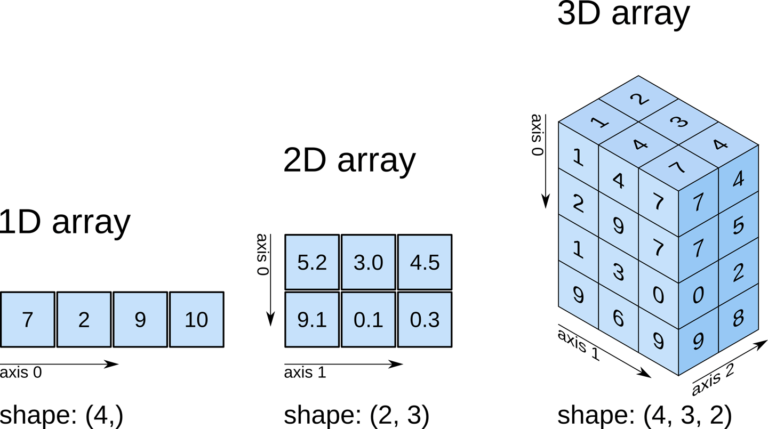
\includegraphics[width=0.5\textwidth]{figures/what-is-numpy-768x429.png}
        \end{center}
    \end{frame}
    \begin{frame}[fragile]{NumPy: N-D array vs Python list}
        \textbf{NumPy: N-D array vs Python list}
        \begin{tabular}{ |p{5.7cm}|p{5.7cm}| }
            \hline
            \textbf{NumPy N-D array} & \textbf{Python list} \\
            \hline
            \begin{itemize}
                \item Fixed-size data structure
                \item Fixed-type elements
                \item Cannot contain ragged sub-arrays
                \item Can be used with mathematical operations
                \item Can be vectorized
            \end{itemize} & \begin{itemize}
                \item Dynamic-size data structure
                \item Can contain any elements of any data type
                \item Can contain ragged sub-lists
                \item Can not be used in mathematical operations
                \item Cannot be vectorized
            \end{itemize} \\
            \hline
        \end{tabular}
    \end{frame}
    \begin{frame}[fragile]{NumPy: Array Creation}
        \begin{example}
            \begin{itemize}
                \item numpy.\textbf{array}([1, 2, 3])
                \item numpy.\textbf{asarray}([1, 2, 3])
                \item numpy.\textbf{asanyarray}([1, 2, 3])
            \end{itemize}
        \end{example}
    \end{frame}
    \begin{frame}[fragile]{NumPy: Array Creation}
        \begin{example}
            \begin{center}
                \begin{tabular}{ | c | p{6.0cm} |}
                    \hline
                    \textbf{Methods} & \textbf{Description} \\
                    \hline
                    numpy.\textbf{empty} & Create an array with uninitialized values \\
                    numpy.\textbf{ones} & Create an array with all values set to 1 \\
                    numpy.\textbf{zeros} & Create an array with all values set to 0 \\
                    numpy.\textbf{full} & Create an array with all values set to a specified value \\
                    \hline
                \end{tabular}
            \end{center}
            % \begin{itemize}
            %     \item numpy.\textbf{empty} Create an array with uninitialized values
            %     \item numpy.\textbf{ones} Create an array with all values set to 1
            %     \item numpy.\textbf{zeros} Create an array with all values set to 0
            %     \item numpy.\textbf{full} Create an array with all values set to a specified value
            % \end{itemize}
        \end{example}
    \end{frame}
    \begin{frame}[fragile]{NumPy: Array Creation}
        \begin{example}
            \begin{center}
                \begin{tabular}{ | c | p{6.0cm} |}
                    \hline
                    \textbf{Methods} & \textbf{Description} \\
                    \hline
                    numpy.\textbf{arange} & Create an array with a range of values \\
                    numpy.\textbf{linspace} & Create an array with equally spaced values \\
                    numpy.\textbf{random.randn} & Create an array from a standard distribution \\
                    numpy.\textbf{random.randint} & Create an array from a uniform distribution \\
                    \hline
                \end{tabular}
            \end{center}
            % \begin{itemize}
            %     \item numpy.\textbf{arange} Create an array with a range of values
            %     \item numpy.\textbf{linspace} Create an array with equally spaced values
            %     \item numpy.\textbf{random.randn} Create an array from a standard distribution
            %     \item numpy.\textbf{random.randint} Create an array from a uniform distribution
            % \end{itemize}
        \end{example}
    \end{frame}

    \begin{frame}[fragile]{NumPy: N-D Indexing}
        \begin{center}
            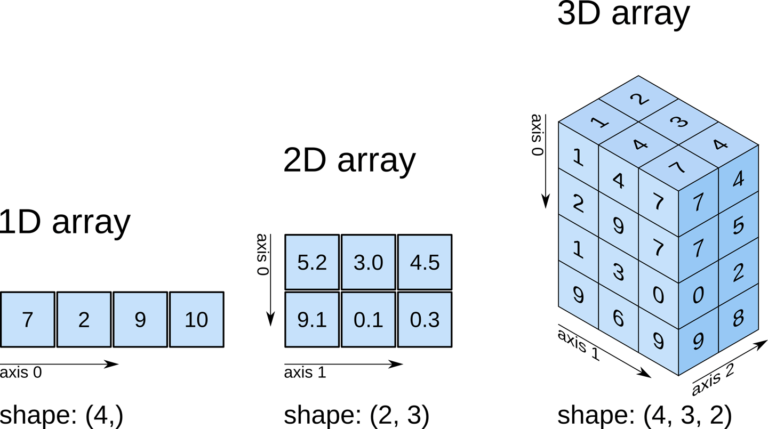
\includegraphics[width=0.5\textwidth]{figures/what-is-numpy-768x429.png}
        \end{center}
    \end{frame}
    \begin{frame}[fragile]{NumPy: N-D Indexing}
        Like Python's native list, a NumPy array can be indexed and sliced using numerical indices. But, unlike Python native Collections, an N-Dimensional NumPy array can be indexed within one set of square brackets.
        \begin{example}
            \begin{lstlisting}[language=Python]
# nested list
a[0][1][2]
#N-D array
a[0,1,2]
            \end{lstlisting}
        \end{example}
    \end{frame}

    \begin{frame}[fragile]{NumPy: N-D Slicing}
        \begin{center}
            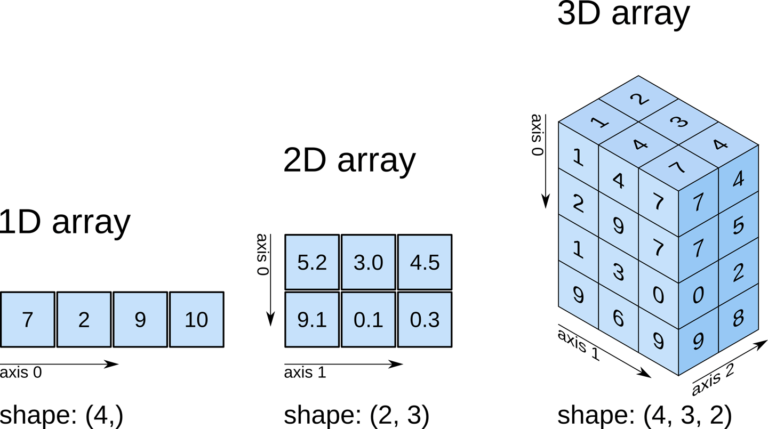
\includegraphics[width=0.5\textwidth]{figures/what-is-numpy-768x429.png}
        \end{center}
    \end{frame}
    \begin{frame}[fragile]{NumPy: N-D Slicing}
        Like indexing, the NumPy array can be sliced using Python's native slicing method. However, unlike the Python native method, the NumPy array supports multidimensional slicing.
        \begin{example}
            \begin{lstlisting}[language=Python]
a[0:2]
a[0:2, 1:3]
a[0:2, ...]
a[0:2, :, :]
            \end{lstlisting}
        \end{example}
        \lstinline[language=Python]{:} denotes the range of slicing. \lstinline[language=Python]{...} denotes the rest of the dimensions.
    \end{frame}

    \begin{frame}[fragile]{NumPy: Masking}
        \begin{center}
            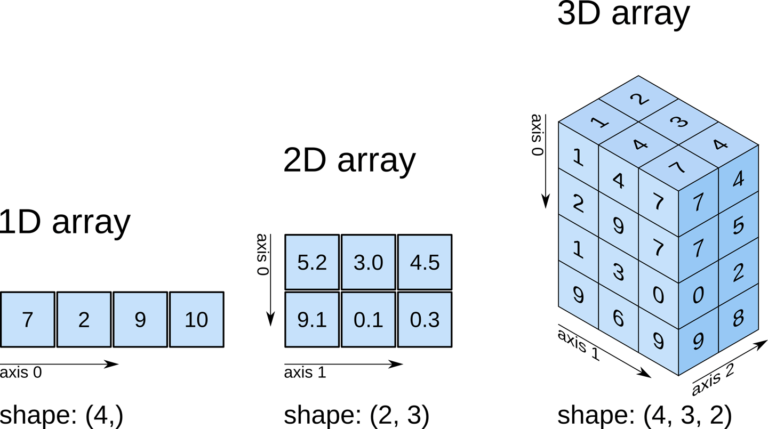
\includegraphics[width=0.5\textwidth]{figures/what-is-numpy-768x429.png}
        \end{center}
    \end{frame}
    \begin{frame}[fragile]{NumPy: Masking \& Indexing}
        Masking is a concept in Numerical Programming where a new boolean array (a mask) is created from an old array using a specified condition.
        \pause
        Mask Indexing is indexing by applying a boolean mask of the same shape and size as indices to the array. Elements with a \lstinline[language=Python]{True} mask are indexed as a result.
        \begin{example}
            \begin{lstlisting}[language=Python]
a = np.array([1, 2, 3, 4, 5])
mask = a > 3 # [False, False, False, True, True]
a[mask] # [4, 5]
            \end{lstlisting}
        \end{example}
    \end{frame}

    \begin{frame}[fragile]{NumPy: Fancy Indexing}
        \begin{center}
            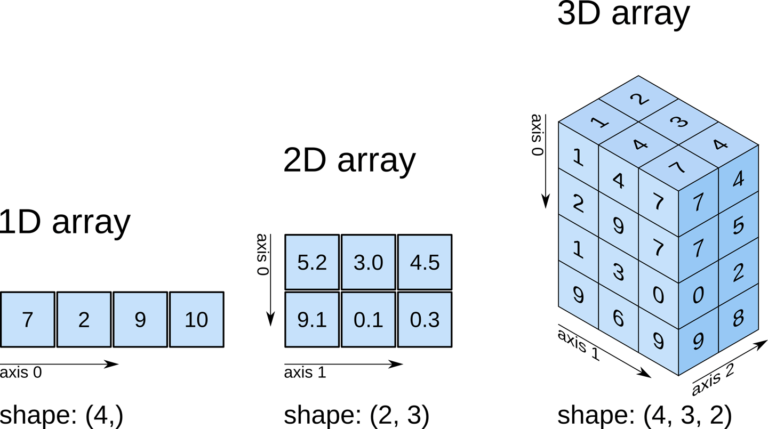
\includegraphics[width=0.5\textwidth]{figures/what-is-numpy-768x429.png}
        \end{center}
    \end{frame}
    \begin{frame}[fragile]{NumPy: Fancy Indexing}
        Aside from mask indexing, NumPy also offers a method known as fancy indexing. In fancy indexing, multiple elements in an array are indexed in one call using another array or other collection. However, unlike slicing, these elements are not required to be contiguous.
        \begin{example}
            \begin{lstlisting}[language=Python]
a = np.array([1, 2, 3, 4, 5])
a[[0, 2, 4]] # [1, 3, 5]
            \end{lstlisting}
        \end{example}
    \end{frame}

    \begin{frame}[fragile]{NumPy: N-D Reshaping}
        Reshaping is a method in NumPy that allows the user to change the shape of an array. The new shape must be compatible with the original shape.
        \begin{example}
            \begin{lstlisting}[language=Python]
a = np.zeros((3, 4, 5))
np.reshape(a, (3, 20)) # reshape to 3x2 array
a.reshape(12, 5) # reshape to 2x3 array
a.reshape(4, -1) # reshape to 3x2 array
            \end{lstlisting}
        \end{example}
    \end{frame}
    \begin{frame}[fragile]{NumPy: Concatenate \& Stack}
        Since NumPy Array's size is fixed at creation, NumPy provides routines to facilitate further modification to the existing array's size by creating a new array using old data.
        \begin{example}
            \begin{center}
                \begin{tabular}{ | c | p{6.0cm} |}
                    \hline
                    \textbf{Methods} & \textbf{Description} \\
                    \hline
                    numpy.\textbf{delete} & Delete elements along the chosen axis from an array \\
                    numpy.\textbf{append} & Append elements to the end of an array \\
                    numpy.\textbf{concatenate} & Join a sequence of arrays along an existing axis \\
                    numpy.\textbf{stack} & Join a sequence of arrays along a new axis \\
                    numpy.\textbf{split} & Split an array into multiple sub-arrays \\
                    \hline
                \end{tabular}
            \end{center}
        \end{example}
    \end{frame}

    \subsubsection{Pandas}
    \begin{frame}[fragile]{Pandas}
        \begin{block}{What is pandas?}
            \begin{itemize}
                \item \textbf{Pandas} is a data analysis and manipulation library that offers comprehensive data structures and data manipulation tools.
                \item \textbf{Pandas} library specializes in analyzing and manipulating numerical tables and time series.
                \item \textbf{Pandas}'s most prominent features include:
                \begin{itemize}
                    \item pandas.\textbf{DataFrame} for indexed data manipulation.
                    \item I/O operation for various file formats.
                    \item Data realignment and imputation.
                    \item Label-based slicing, fancy indexing, and subsetting of large data sets.
                    \item SQL-like internal analytic engine
                \end{itemize}
            \end{itemize}
        \end{block}
    \end{frame}
    \begin{frame}[fragile]{Pandas: DataFrame}
        \begin{block}{Pandas: DataFrame}
            \begin{itemize}
                \item A DataFrame is a two-dimensional, size-mutable, potentially heterogeneous tabular data structure with labeled axes (rows and columns).
                \item A DataFrame is similar to a spreadsheet or SQL table or a dictionary of Series objects.
                \item The DataFrame is generally the most commonly used pandas object.
            \end{itemize}
        \end{block}
    \end{frame}

    \begin{frame}[fragile]
    \frametitle{Descriptive statistics with Pandas}
    \begin{lstlisting}[caption=Calculating the average and standard deviation of a column using Pandas][language=Python]
average = data['A'].mean()
std_dev = data['A'].std()
print("Average of column A:", average)
print("Standard deviation of column A:", std_dev)
    \end{lstlisting}
    \end{frame}
%     \begin{frame}[fragile]
%         \frametitle{How distributed is the data?}
%         \begin{itemize}
%             \item \textbf{Histogram} is a graphical plot that shows the distribution of a numeric variable's values as a series of bars; each bar represents the frequency of the corresponding interval or bin of the data.
%             \item \textbf{Box plot} is a graphical representation of a dataset summarising its distribution in five key statistics: the minimum and maximum values, the lower and upper quartiles, and the median.
%         \end{itemize}
%     \end{frame}

%     \begin{frame}[fragile]
%         \frametitle{Histograms}
%         \begin{lstlisting}[language=Python]
% import matplotlib.pyplot as plt

% # Create a list of ages

% ages = [18, 22, 25, 28, 32, 35, 38, 41, 45, 48, 52, 55, 58, 62]

% # Define the bin edges

% bin_edges = [18, 30, 40, 50, 62]

% # Create an empty list for the bin counts

% bin_counts = [0, 0, 0, 0]
%         \end{lstlisting}
%     \end{frame}
\end{document}